%%% Template originaly created by Karol Kozioł (mail@karol-koziol.net) and modified for ShareLaTeX use

\documentclass[a4paper,11pt]{article}

\usepackage[T1]{fontenc}
\usepackage[utf8]{inputenc}
\usepackage{graphicx}
\usepackage{xcolor}

\renewcommand\familydefault{\sfdefault}
\usepackage{tgheros}
\usepackage[defaultmono]{droidmono}

\usepackage{amsmath,amssymb,amsthm,textcomp}
\usepackage{enumerate}
\usepackage{multicol}
\usepackage{tikz}

\usepackage{geometry}
\geometry{left=25mm,right=25mm,%
bindingoffset=0mm, top=20mm,bottom=20mm}

\usepackage[export]{adjustbox}
\usepackage{subcaption}
\usepackage{float}


\linespread{1.3}

\newcommand{\linia}{\rule{\linewidth}{0.5pt}}

% custom theorems if needed
\newtheoremstyle{mytheor}
    {1ex}{1ex}{\normalfont}{0pt}{\scshape}{.}{1ex}
    {{\thmname{#1 }}{\thmnumber{#2}}{\thmnote{ (#3)}}}

\theoremstyle{mytheor}
\newtheorem{defi}{Definition}

% my own titles
\makeatletter
\renewcommand{\maketitle}{
\begin{center}
\vspace{2ex}
{\huge \textsc{\@title}}
\vspace{1ex}
\\
\linia\\
\@author \hfill \@date
\vspace{4ex}
\end{center}
}
\makeatother
%%%

% custom footers and headers
\usepackage{fancyhdr}
\pagestyle{fancy}
\lhead{}
\chead{}
\rhead{}
\lfoot{Analiza Algorytmów, lab 3}
\cfoot{}
\rfoot{Page \thepage}
\renewcommand{\headrulewidth}{0pt}
\renewcommand{\footrulewidth}{0pt}
%

\graphicspath{ {../png/} }

%%%----------%%%----------%%%----------%%%----------%%%

\begin{document}

\title{Analiza Algorytmów, lab 3}

\author{Adrian Mucha, Politechnika Wrocławska, WPPT}

\date{25/04/2020}

\maketitle

\section*{Zad 9}

Generowane multizbiory (każdy eksperyment, dla każdego $n$) zawierają zdarzenia niezależne od siebie. Każdy element posiada unikalne \texttt{id}, które są kolejnymi liczbami naturalnymi.

Wartości cech są generowane według zdefiniowanych parametryzowanych strategii, które zostały podzielone na sekcje i opisane poniżej.

Do uzyskania losowości funkcji haszującej rzutującej na zbiór $[0, 1]$ użyto funkcji \texttt{md5}, \texttt{sha1}, \texttt{sha3}. Zbadano wyniki dla różnych wartości parametru $m$ oznaczającego ilość rejestrów.

Zgodnie z intuicją, obserwujemy że im większy parametr $m$, tym dokładniejsze są wartości aproksymacji sumy.

Dobrane funkcje haszujące nie dają różnicy pomiędzy eksperymentami. Należy jednak zaznaczyć, że ich odporność na kolizje ma znaczący wpływ na ogólną precyzję algorytmu.

\subsection*{Nierówność Czebyszewa}
\begin{gather*}
    P(|X - \mathbb{E}(X)| < \delta) > 1 - \alpha \\
    X = \frac{\hat{\Lambda}}{\Lambda}, \mathbb{E}(X) = 1 \\
    \alpha = \frac{\text{Var}(\frac{\hat{\Lambda}}{\Lambda})}{\delta^2}, 
    \text{Var}(\frac{\hat{\Lambda}}{\Lambda}) = \frac{1}{m - 2} \\
    \alpha = \frac{\frac{1}{m - 2}}{\delta^2}, 
    \delta = \sqrt{\frac{1}{\alpha(m - 2)}}
\end{gather*}
\begin{figure}[H]
    \begin{subfigure}{0.32\textwidth}
        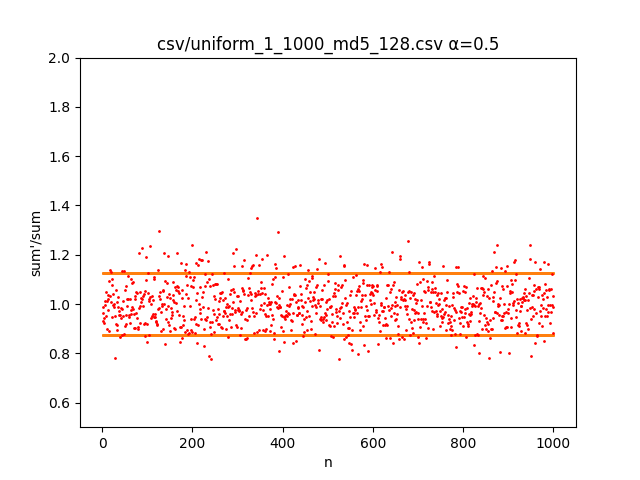
\includegraphics[width=1.0\linewidth, height=5cm]{czebyszew/uniform_1_1000_md5_128_m_128_a_0_5.png}
        \caption{$\alpha = 0.5$}
        \label{fig:subim2}
    \end{subfigure}
    \begin{subfigure}{0.32\textwidth}
        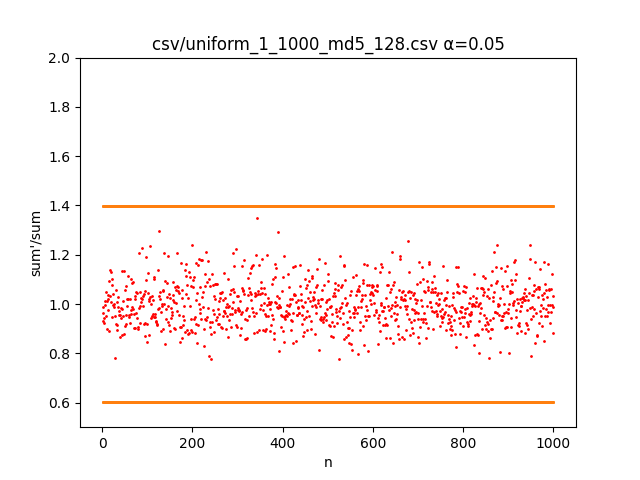
\includegraphics[width=1.0\linewidth, height=5cm]{czebyszew/uniform_1_1000_md5_128_m_128_a_0_05.png}
        \caption{$\alpha = 0.05$}
        \label{fig:subim2}
    \end{subfigure}
    \begin{subfigure}{0.32\textwidth}
        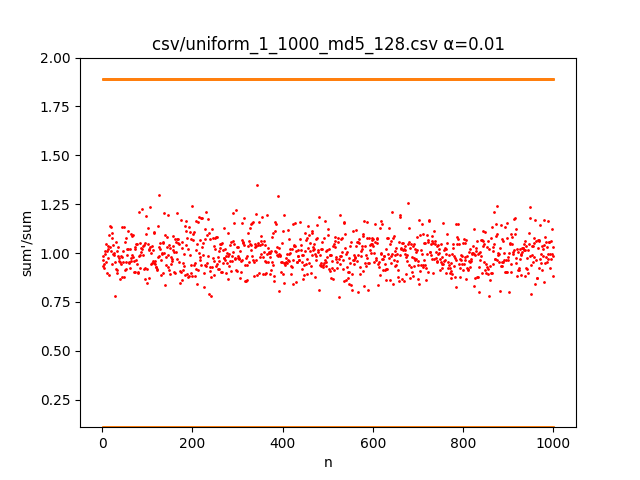
\includegraphics[width=1.0\linewidth, height=5cm]{czebyszew/uniform_1_1000_md5_128_m_128_a_0_01.png}
        \caption{$\alpha = 0.1$}
        \label{fig:subim2}
    \end{subfigure}

    \caption{Wykresy przedstawiają nierówności Czebyszewa nałożone na wykresy z różnymi parametrami $\alpha$. Możemy zaobserwować, że ograniczenia uzyskane z nierówności prawidłowo odzwierciedlają otrzymane wyniki.}
    \label{fig:uniform_md5}
\end{figure}

\subsection*{Rozkład jednostajny na $[1, 1000]$}
Strategia generowania cech, to próbkowanie z zakresu $[1, 1000]$.
\begin{figure}[H]
    \begin{subfigure}{0.5\textwidth}
        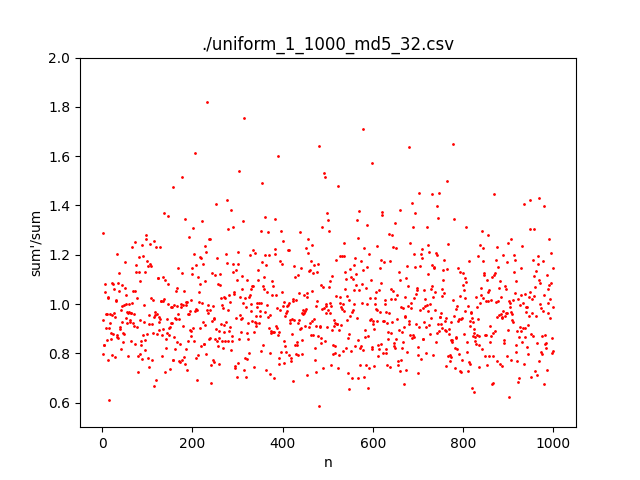
\includegraphics[width=1.0\linewidth, height=5cm]{uniform_1_1000/uniform_1_1000_md5_32.png}
        \caption{$m = 32$}
        \label{fig:subim1}
    \end{subfigure}
    \begin{subfigure}{0.5\textwidth}
        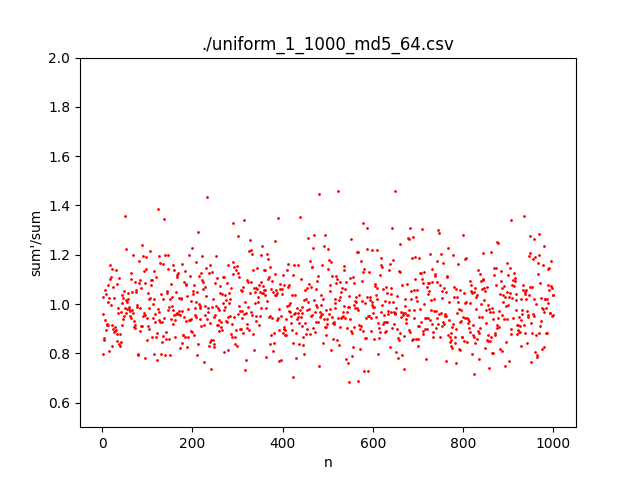
\includegraphics[width=1.0\linewidth, height=5cm]{uniform_1_1000/uniform_1_1000_md5_64.png}
        \caption{$m = 64$}
        \label{fig:subim1}
    \end{subfigure}
    \begin{subfigure}{0.5\textwidth}
        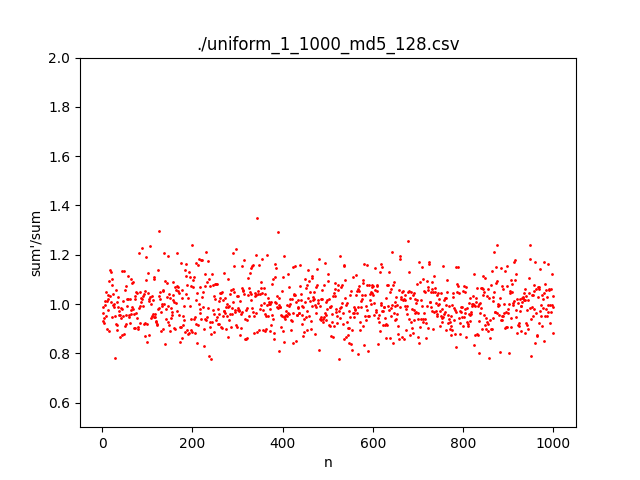
\includegraphics[width=1.0\linewidth, height=5cm]{uniform_1_1000/uniform_1_1000_md5_128.png}
        \caption{$m = 128$}
        \label{fig:subim2}
    \end{subfigure}
    \begin{subfigure}{0.5\textwidth}
        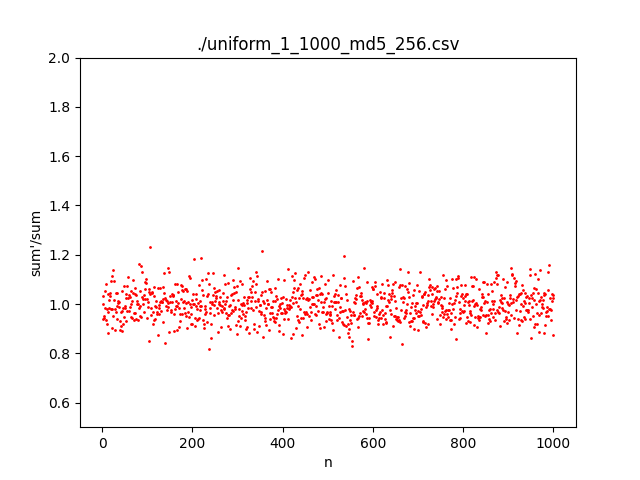
\includegraphics[width=1.0\linewidth, height=5cm]{uniform_1_1000/uniform_1_1000_md5_256.png}
        \caption{$m = 256$}
        \label{fig:subim2}
    \end{subfigure}

    \caption{Wykresy przedstawiają wyniki algorytmu dla różnej ilości rejestrów gdy wartości cech pochodzą z rozkładu jednostajnego na przedziale $[1, 1000]$. Wykorzystany algorytm: \texttt{md5}.}
    \label{fig:uniform_md5}
\end{figure}

\begin{figure}[H]
    \begin{subfigure}{0.5\textwidth}
        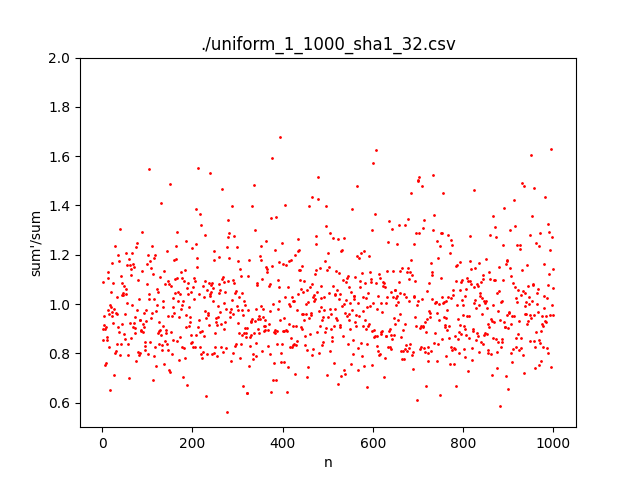
\includegraphics[width=1.0\linewidth, height=5cm]{uniform_1_1000/uniform_1_1000_sha1_32.png}
        \caption{$m = 32$}
        \label{fig:subim1}
    \end{subfigure}
    \begin{subfigure}{0.5\textwidth}
        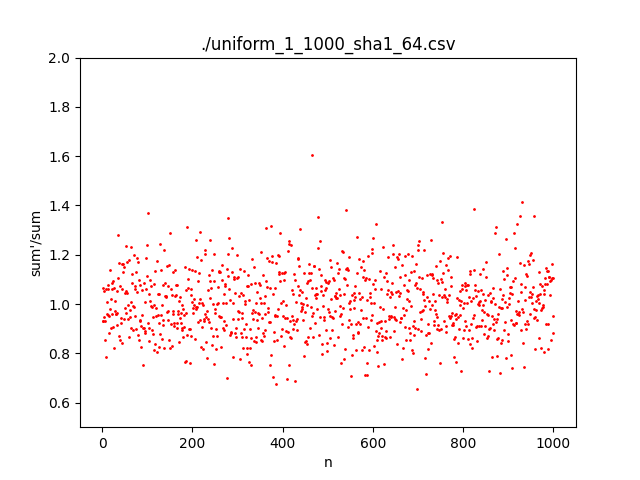
\includegraphics[width=1.0\linewidth, height=5cm]{uniform_1_1000/uniform_1_1000_sha1_64.png}
        \caption{$m = 64$}
        \label{fig:subim1}
    \end{subfigure}
    \begin{subfigure}{0.5\textwidth}
        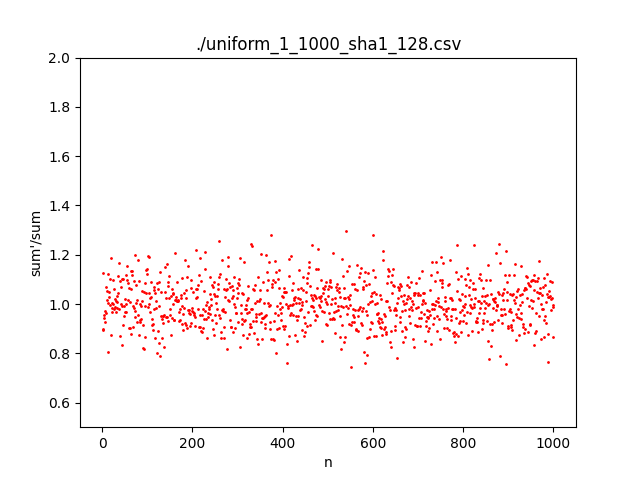
\includegraphics[width=1.0\linewidth, height=5cm]{uniform_1_1000/uniform_1_1000_sha1_128.png}
        \caption{$m = 128$}
        \label{fig:subim2}
    \end{subfigure}
    \begin{subfigure}{0.5\textwidth}
        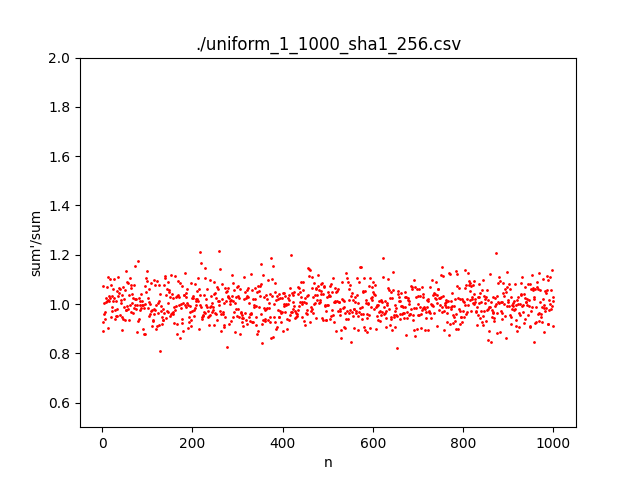
\includegraphics[width=1.0\linewidth, height=5cm]{uniform_1_1000/uniform_1_1000_sha1_256.png}
        \caption{$m = 256$}
        \label{fig:subim2}
    \end{subfigure}

    \caption{Wykresy przedstawiają wyniki algorytmu dla różnej ilości rejestrów gdy wartości cech pochodzą z rozkładu jednostajnego na przedziale $[1, 1000]$. Wykorzystany algorytm: \texttt{sha1}.}
    \label{fig:uniform_sha1}
\end{figure}

\begin{figure}[H]
    \begin{subfigure}{0.5\textwidth}
        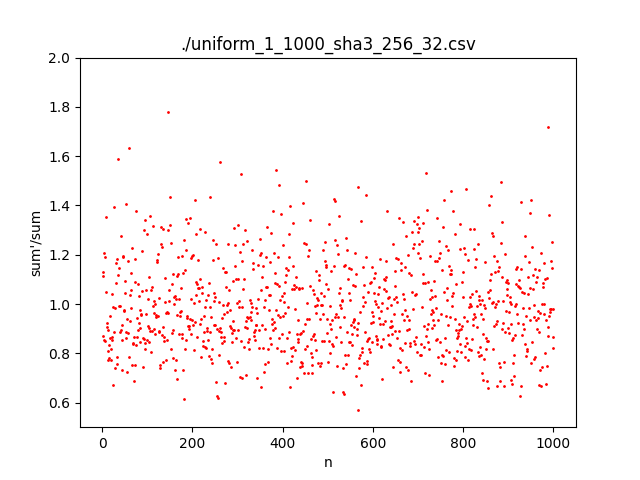
\includegraphics[width=1.0\linewidth, height=5cm]{uniform_1_1000/uniform_1_1000_sha3_256_32.png}
        \caption{$m = 32$}
        \label{fig:subim1}
    \end{subfigure}
    \begin{subfigure}{0.5\textwidth}
        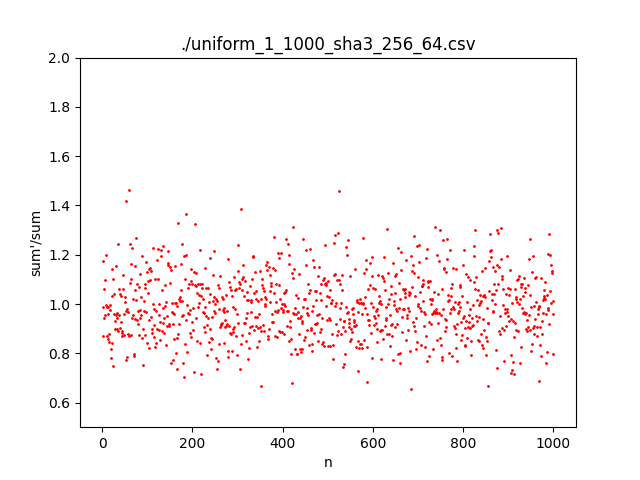
\includegraphics[width=1.0\linewidth, height=5cm]{uniform_1_1000/uniform_1_1000_sha3_256_64.png}
        \caption{$m = 64$}
        \label{fig:subim1}
    \end{subfigure}
    \begin{subfigure}{0.5\textwidth}
        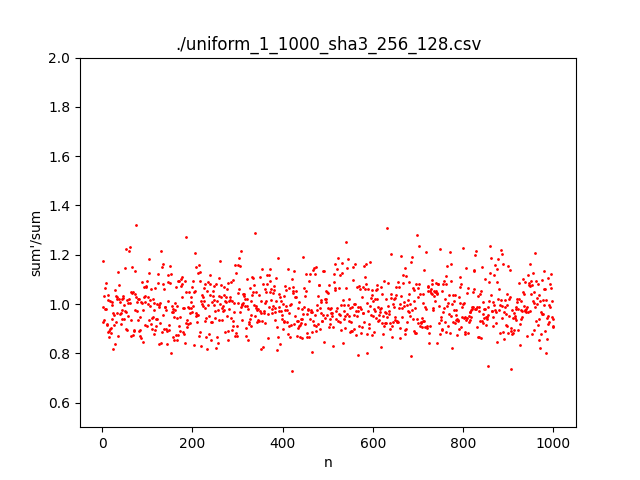
\includegraphics[width=1.0\linewidth, height=5cm]{uniform_1_1000/uniform_1_1000_sha3_256_128.png}
        \caption{$m = 128$}
        \label{fig:subim2}
    \end{subfigure}
    \begin{subfigure}{0.5\textwidth}
        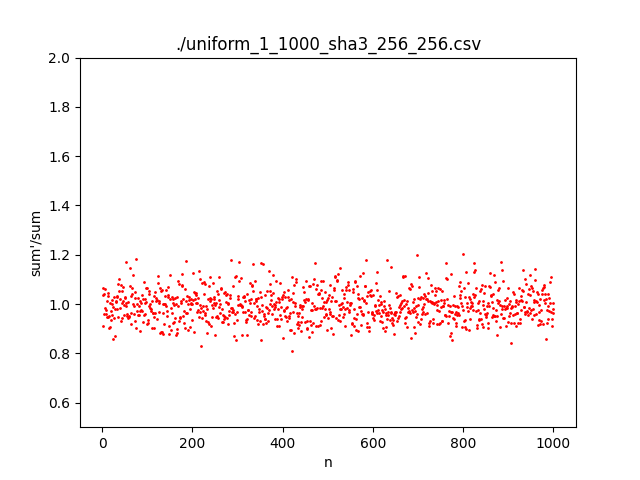
\includegraphics[width=1.0\linewidth, height=5cm]{uniform_1_1000/uniform_1_1000_sha3_256_256.png}
        \caption{$m = 256$}
        \label{fig:subim2}
    \end{subfigure}

    \caption{Wykresy przedstawiają wyniki algorytmu dla różnej ilości rejestrów gdy wartości cech pochodzą z rozkładu jednostajnego na przedziale $[1, 1000]$. Wykorzystany algorytm: \texttt{sha3}.}
    \label{fig:uniform_sha3_256}
\end{figure}


\subsection*{Rozkład jednostajny na $[400, 600]$}
Strategia generowania cech, to próbkowanie z zakresu $[400, 600]$. Brak znaczących różnic w porównaniu do zbioru $[1, 1000]$.
\begin{figure}[H]
    \begin{subfigure}{0.5\textwidth}
        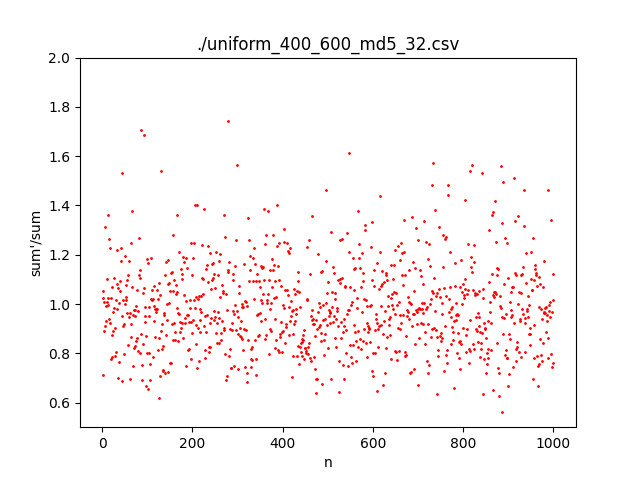
\includegraphics[width=1.0\linewidth, height=5cm]{uniform_400_600/uniform_400_600_md5_32.png}
        \caption{$m = 32$}
        \label{fig:subim1}
    \end{subfigure}
    \begin{subfigure}{0.5\textwidth}
        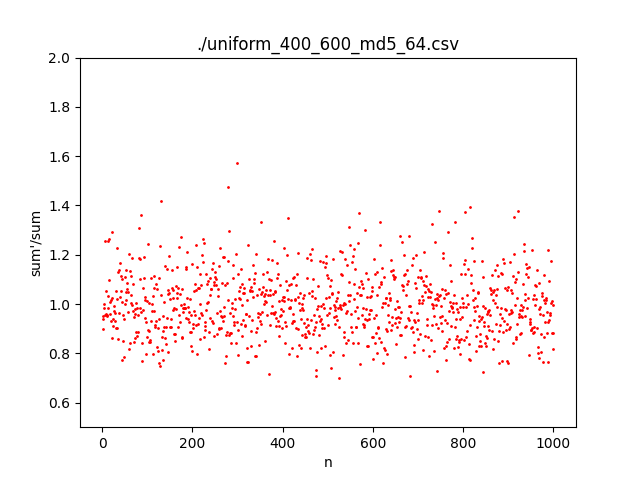
\includegraphics[width=1.0\linewidth, height=5cm]{uniform_400_600/uniform_400_600_md5_64.png}
        \caption{$m = 64$}
        \label{fig:subim1}
    \end{subfigure}
    \begin{subfigure}{0.5\textwidth}
        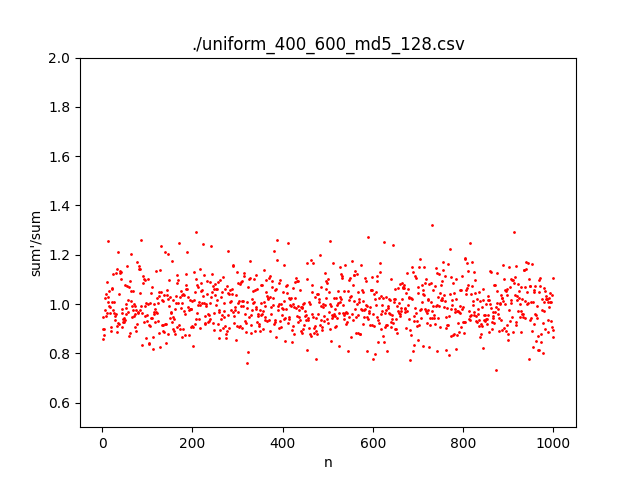
\includegraphics[width=1.0\linewidth, height=5cm]{uniform_400_600/uniform_400_600_md5_128.png}
        \caption{$m = 128$}
        \label{fig:subim2}
    \end{subfigure}
    \begin{subfigure}{0.5\textwidth}
        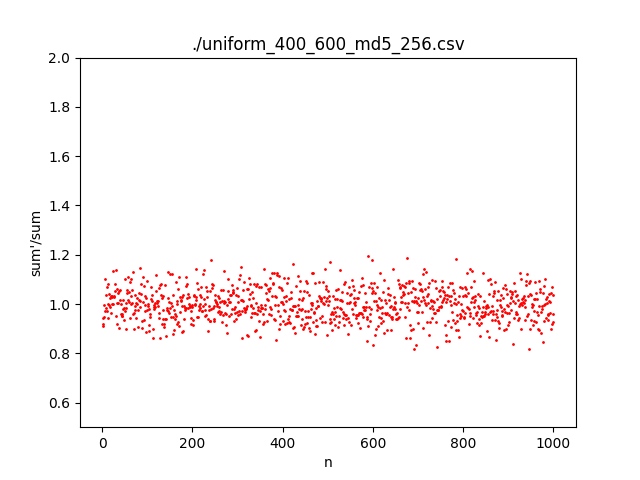
\includegraphics[width=1.0\linewidth, height=5cm]{uniform_400_600/uniform_400_600_md5_256.png}
        \caption{$m = 256$}
        \label{fig:subim2}
    \end{subfigure}

    \caption{Wykresy przedstawiają wyniki algorytmu dla różnej ilości rejestrów gdy wartości cech pochodzą z rozkładu jednostajnego na przedziale $[400, 600]$. Wykorzystany algorytm: \texttt{md5}.}
    \label{fig:uniform_md5}
\end{figure}

\begin{figure}[H]
    \begin{subfigure}{0.5\textwidth}
        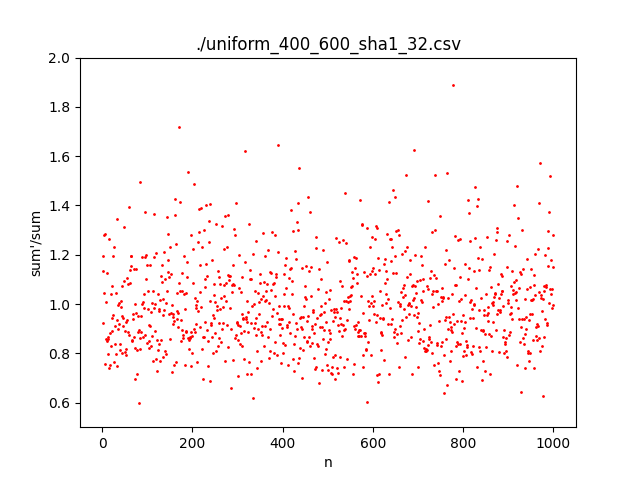
\includegraphics[width=1.0\linewidth, height=5cm]{uniform_400_600/uniform_400_600_sha1_32.png}
        \caption{$m = 32$}
        \label{fig:subim1}
    \end{subfigure}
    \begin{subfigure}{0.5\textwidth}
        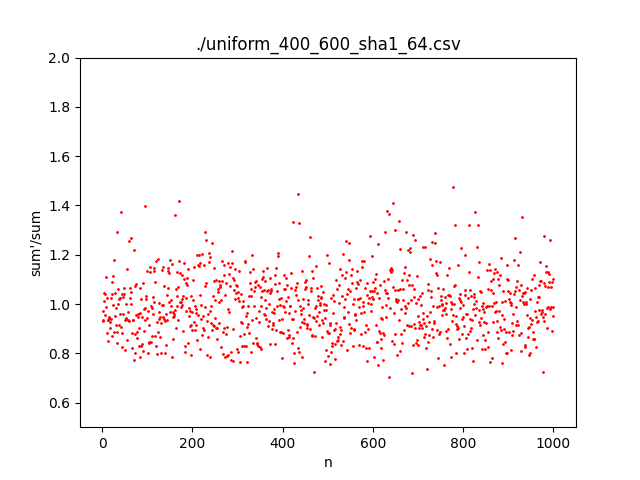
\includegraphics[width=1.0\linewidth, height=5cm]{uniform_400_600/uniform_400_600_sha1_64.png}
        \caption{$m = 64$}
        \label{fig:subim1}
    \end{subfigure}
    \begin{subfigure}{0.5\textwidth}
        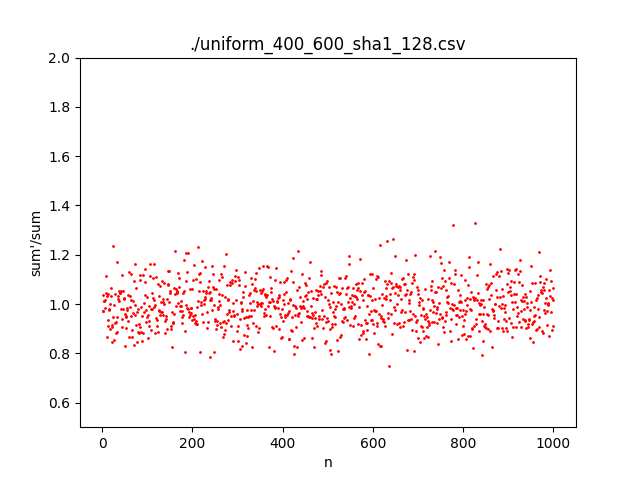
\includegraphics[width=1.0\linewidth, height=5cm]{uniform_400_600/uniform_400_600_sha1_128.png}
        \caption{$m = 128$}
        \label{fig:subim2}
    \end{subfigure}
    \begin{subfigure}{0.5\textwidth}
        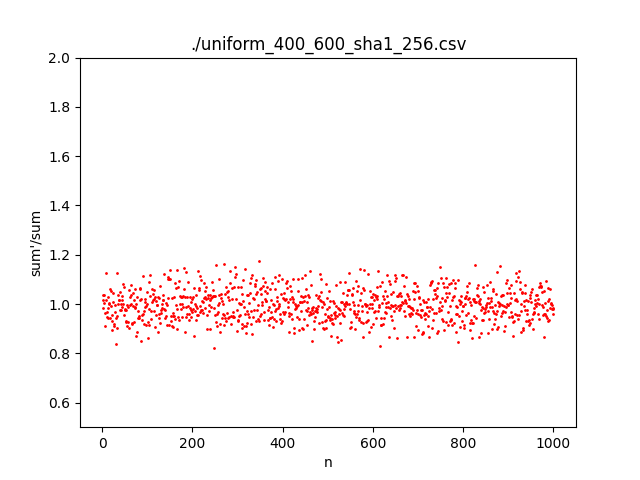
\includegraphics[width=1.0\linewidth, height=5cm]{uniform_400_600/uniform_400_600_sha1_256.png}
        \caption{$m = 256$}
        \label{fig:subim2}
    \end{subfigure}

    \caption{Wykresy przedstawiają wyniki algorytmu dla różnej ilości rejestrów gdy wartości cech pochodzą z rozkładu jednostajnego na przedziale $[400, 600]$. Wykorzystany algorytm: \texttt{sha1}.}
    \label{fig:uniform_sha1}
\end{figure}

\begin{figure}[H]
    \begin{subfigure}{0.5\textwidth}
        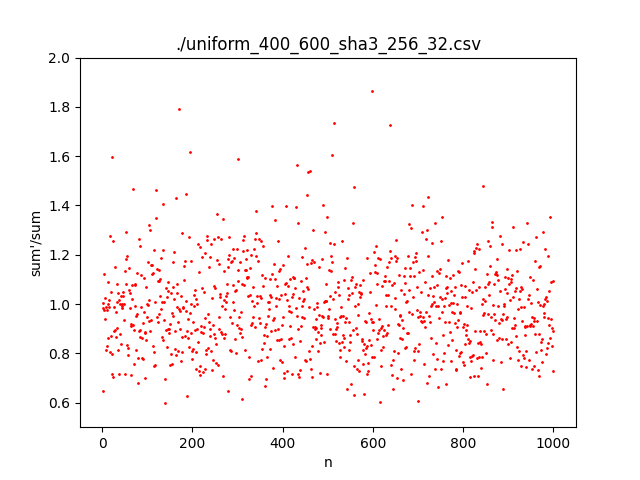
\includegraphics[width=1.0\linewidth, height=5cm]{uniform_400_600/uniform_400_600_sha3_256_32.png}
        \caption{$m = 32$}
        \label{fig:subim1}
    \end{subfigure}
    \begin{subfigure}{0.5\textwidth}
        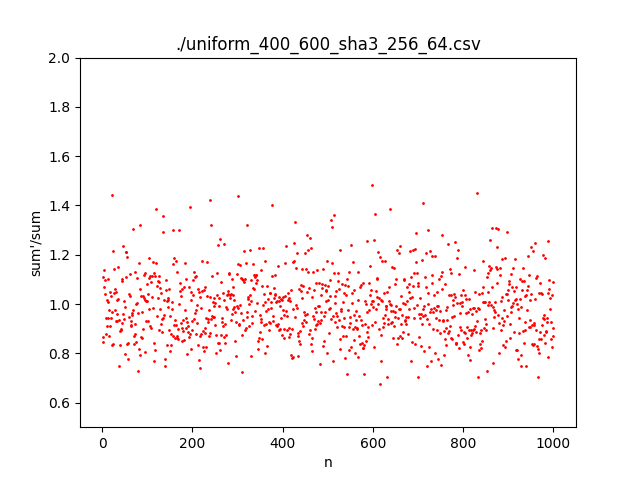
\includegraphics[width=1.0\linewidth, height=5cm]{uniform_400_600/uniform_400_600_sha3_256_64.png}
        \caption{$m = 64$}
        \label{fig:subim1}
    \end{subfigure}
    \begin{subfigure}{0.5\textwidth}
        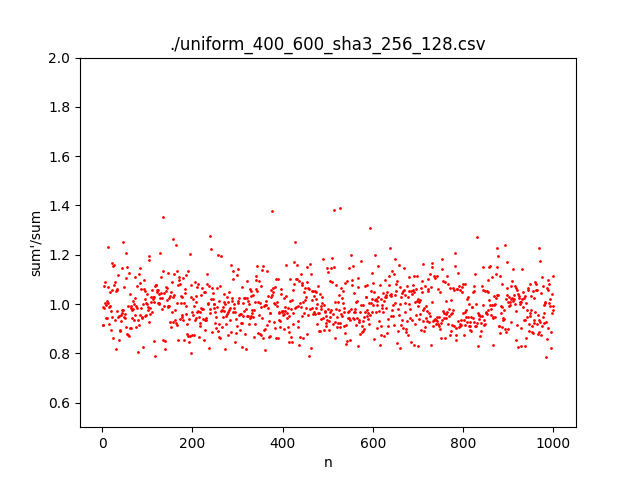
\includegraphics[width=1.0\linewidth, height=5cm]{uniform_400_600/uniform_400_600_sha3_256_128.png}
        \caption{$m = 128$}
        \label{fig:subim2}
    \end{subfigure}
    \begin{subfigure}{0.5\textwidth}
        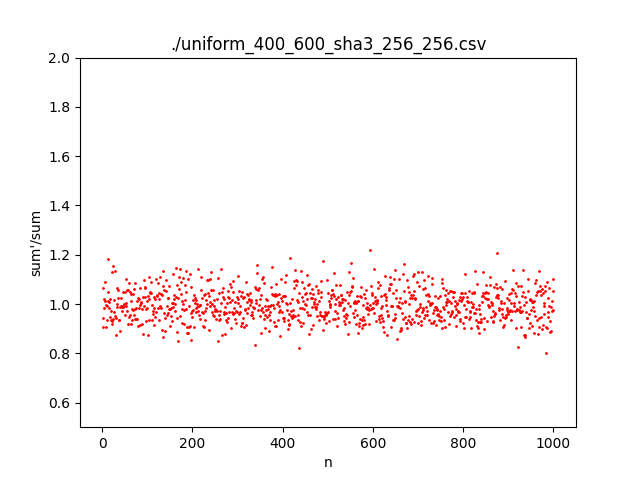
\includegraphics[width=1.0\linewidth, height=5cm]{uniform_400_600/uniform_400_600_sha3_256_256.png}
        \caption{$m = 256$}
        \label{fig:subim2}
    \end{subfigure}

    \caption{Wykresy przedstawiają wyniki algorytmu dla różnej ilości rejestrów gdy wartości cech pochodzą z rozkładu jednostajnego na przedziale $[400, 600]$. Wykorzystany algorytm: \texttt{sha3}.}
    \label{fig:uniform_sha3_256}
\end{figure}


\subsection*{Jednakowe cechy}
W tej strategii wszystkie cechy są ustawione na $1$. W tym przypadku algorytm zachowuje się podobnie jak \texttt{MinCount} i zlicza unikalne wystąpienia, lecz daje gorsze wyniki.
\begin{figure}[H]
    \begin{subfigure}{0.5\textwidth}
        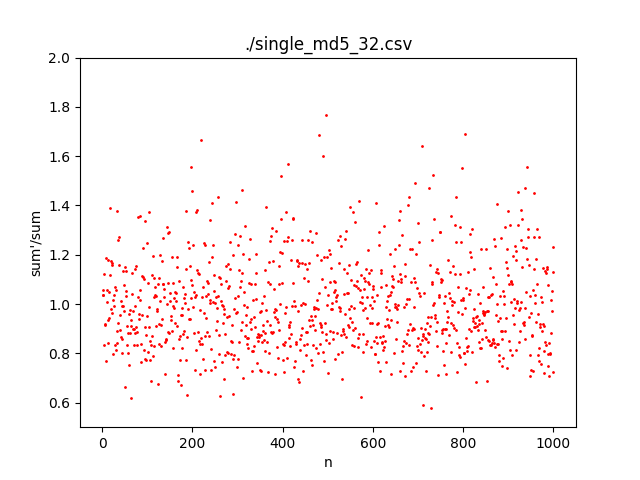
\includegraphics[width=1.0\linewidth, height=5cm]{single/single_md5_32.png}
        \caption{$m = 32$}
        \label{fig:subim1}
    \end{subfigure}
    \begin{subfigure}{0.5\textwidth}
        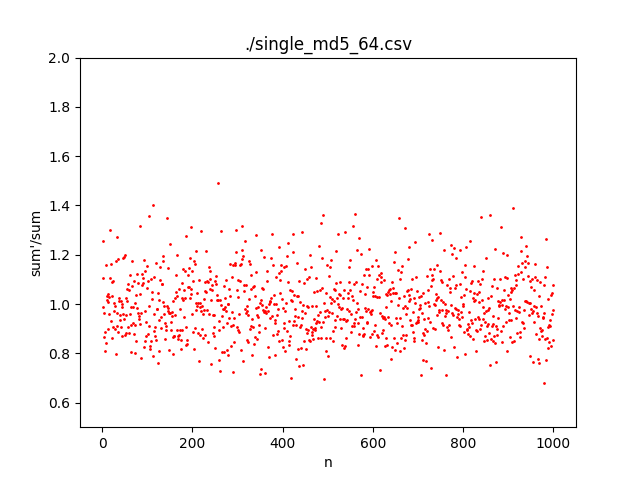
\includegraphics[width=1.0\linewidth, height=5cm]{single/single_md5_64.png}
        \caption{$m = 64$}
        \label{fig:subim1}
    \end{subfigure}
    \begin{subfigure}{0.5\textwidth}
        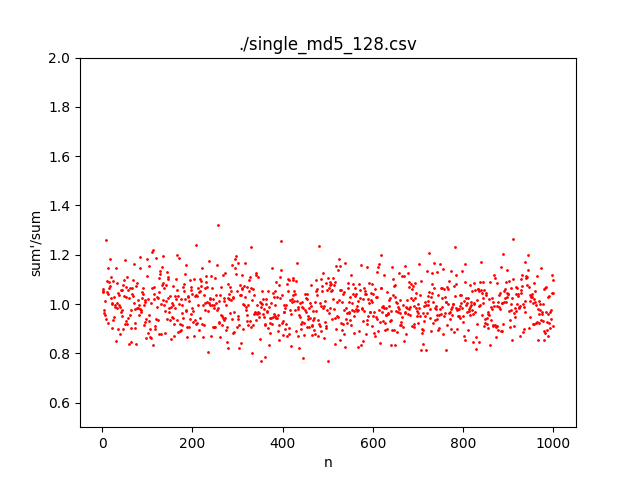
\includegraphics[width=1.0\linewidth, height=5cm]{single/single_md5_128.png}
        \caption{$m = 128$}
        \label{fig:subim2}
    \end{subfigure}
    \begin{subfigure}{0.5\textwidth}
        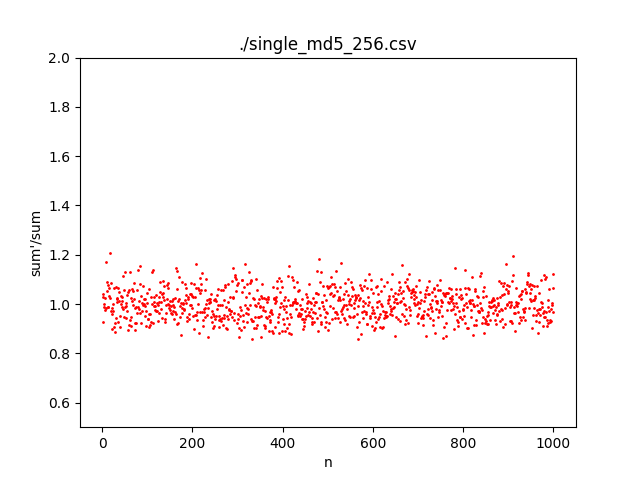
\includegraphics[width=1.0\linewidth, height=5cm]{single/single_md5_256.png}
        \caption{$m = 256$}
        \label{fig:subim2}
    \end{subfigure}

    \caption{Wykresy przedstawiają wyniki algorytmu dla różnej ilości rejestrów gdy wartości cech są jednakowe (wynoszą $1$). Wykorzystany algorytm: \texttt{md5}.}
    \label{fig:uniform_md5}
\end{figure}

\begin{figure}[H]
    \begin{subfigure}{0.5\textwidth}
        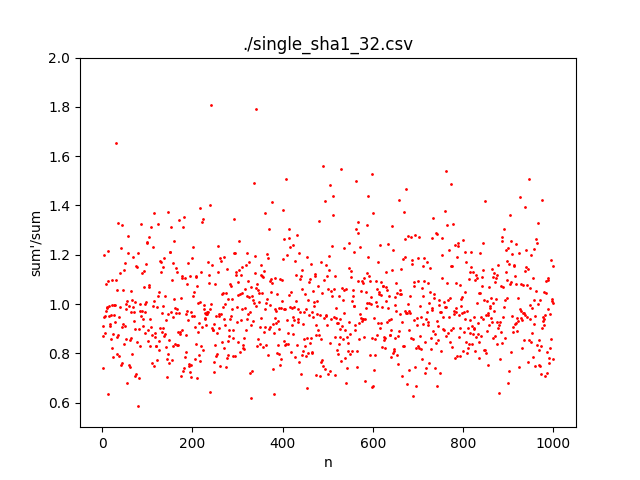
\includegraphics[width=1.0\linewidth, height=5cm]{single/single_sha1_32.png}
        \caption{$m = 32$}
        \label{fig:subim1}
    \end{subfigure}
    \begin{subfigure}{0.5\textwidth}
        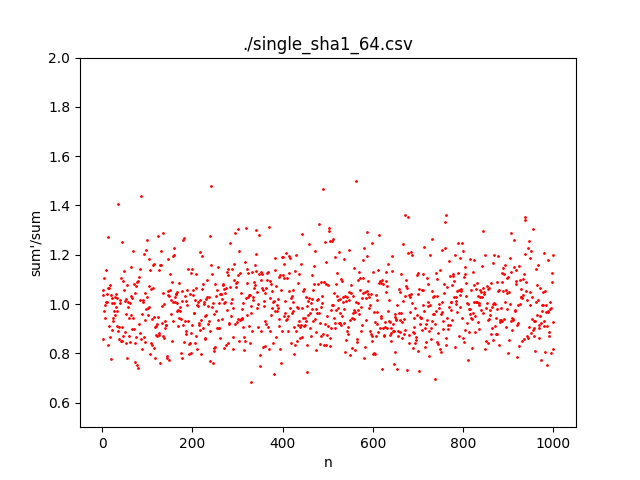
\includegraphics[width=1.0\linewidth, height=5cm]{single/single_sha1_64.png}
        \caption{$m = 64$}
        \label{fig:subim1}
    \end{subfigure}
    \begin{subfigure}{0.5\textwidth}
        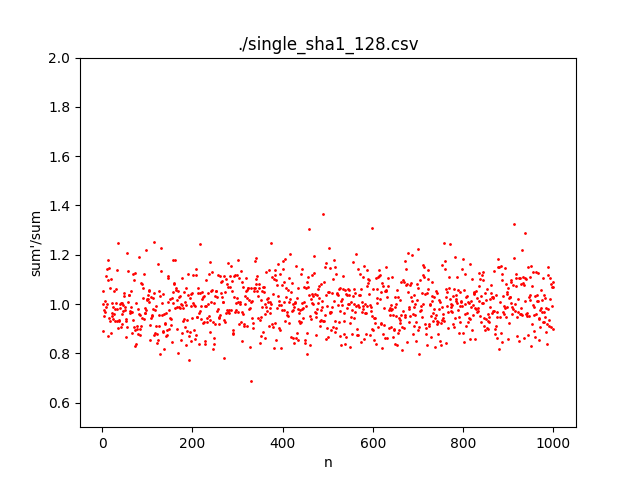
\includegraphics[width=1.0\linewidth, height=5cm]{single/single_sha1_128.png}
        \caption{$m = 128$}
        \label{fig:subim2}
    \end{subfigure}
    \begin{subfigure}{0.5\textwidth}
        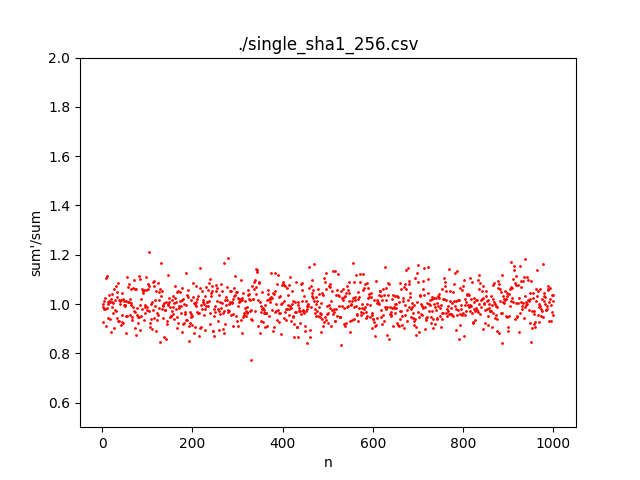
\includegraphics[width=1.0\linewidth, height=5cm]{single/single_sha1_256.png}
        \caption{$m = 256$}
        \label{fig:subim2}
    \end{subfigure}

    \caption{Wykresy przedstawiają wyniki algorytmu dla różnej ilości rejestrów gdy wartości cech są jednakowe (wynoszą $1$). Wykorzystany algorytm: \texttt{sha1}.}
    \label{fig:uniform_sha1}
\end{figure}

\begin{figure}[H]
    \begin{subfigure}{0.5\textwidth}
        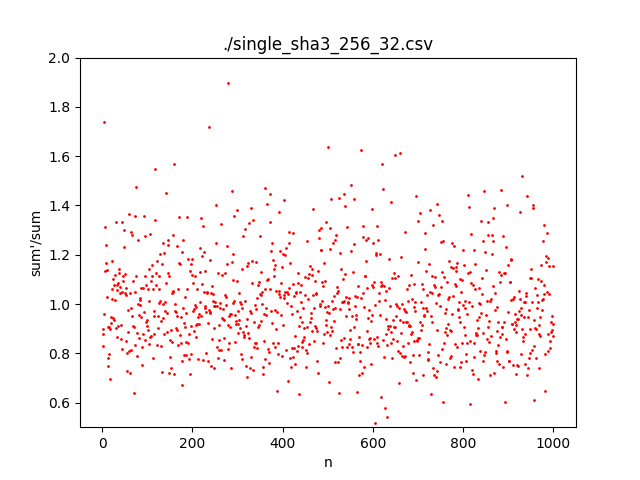
\includegraphics[width=1.0\linewidth, height=5cm]{single/single_sha3_256_32.png}
        \caption{$m = 32$}
        \label{fig:subim1}
    \end{subfigure}
    \begin{subfigure}{0.5\textwidth}
        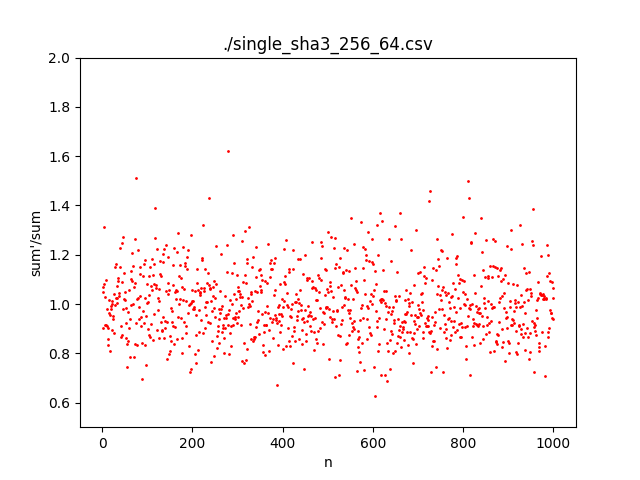
\includegraphics[width=1.0\linewidth, height=5cm]{single/single_sha3_256_64.png}
        \caption{$m = 64$}
        \label{fig:subim1}
    \end{subfigure}
    \begin{subfigure}{0.5\textwidth}
        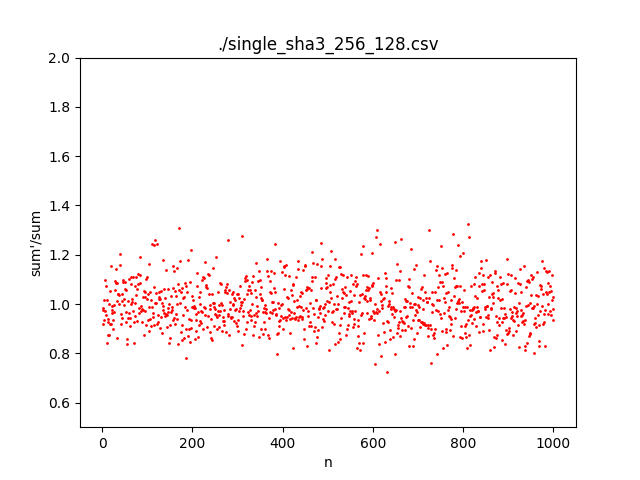
\includegraphics[width=1.0\linewidth, height=5cm]{single/single_sha3_256_128.png}
        \caption{$m = 128$}
        \label{fig:subim2}
    \end{subfigure}
    \begin{subfigure}{0.5\textwidth}
        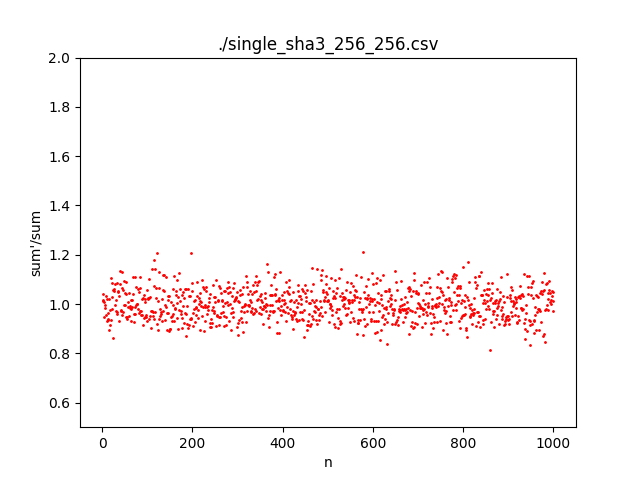
\includegraphics[width=1.0\linewidth, height=5cm]{single/single_sha3_256_256.png}
        \caption{$m = 256$}
        \label{fig:subim2}
    \end{subfigure}

    \caption{Wykresy przedstawiają wyniki algorytmu dla różnej ilości rejestrów gdy wartości cech są jednakowe (wynoszą $1$). Wykorzystany algorytm: \texttt{sha3}.}
    \label{fig:uniform_sha3_256}
\end{figure}


\subsection*{Wartości odstające}
Wartość cechy losowana jest ze zbioru $[1,2,1,2,\ldots]$, którego $1\%$ stanowi wartość odstająca (duża liczba, np. $1000$).
\begin{figure}[H]
    \begin{subfigure}{0.5\textwidth}
        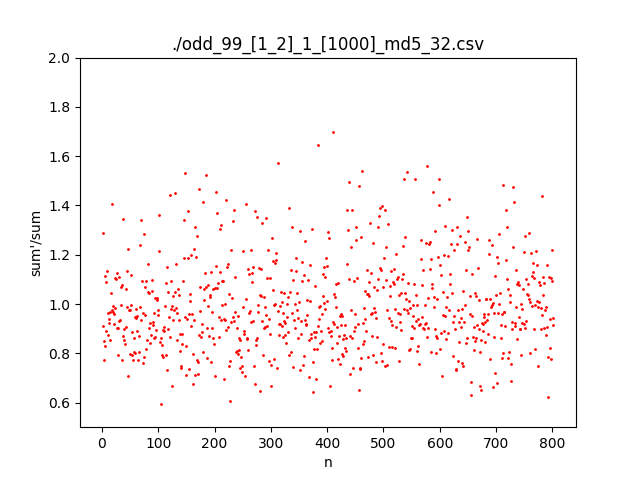
\includegraphics[width=1.0\linewidth, height=5cm]{odd_99_1_2_1_1000/odd_99_1_2_1_1000_md5_32.png}
        \caption{$m = 32$}
        \label{fig:subim1}
    \end{subfigure}
    \begin{subfigure}{0.5\textwidth}
        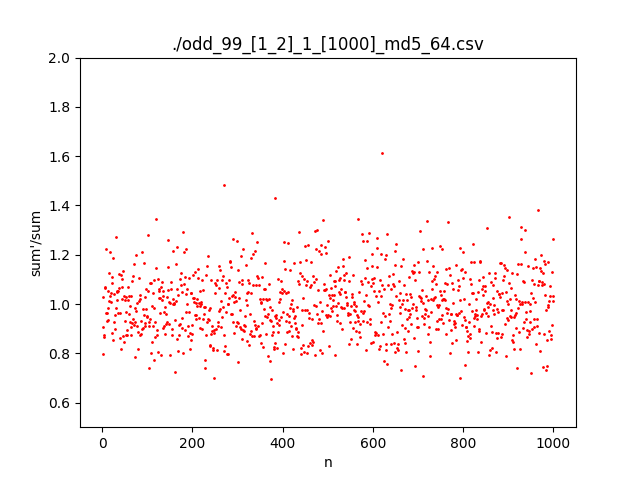
\includegraphics[width=1.0\linewidth, height=5cm]{odd_99_1_2_1_1000/odd_99_1_2_1_1000_md5_64.png}
        \caption{$m = 64$}
        \label{fig:subim1}
    \end{subfigure}
    \begin{subfigure}{0.5\textwidth}
        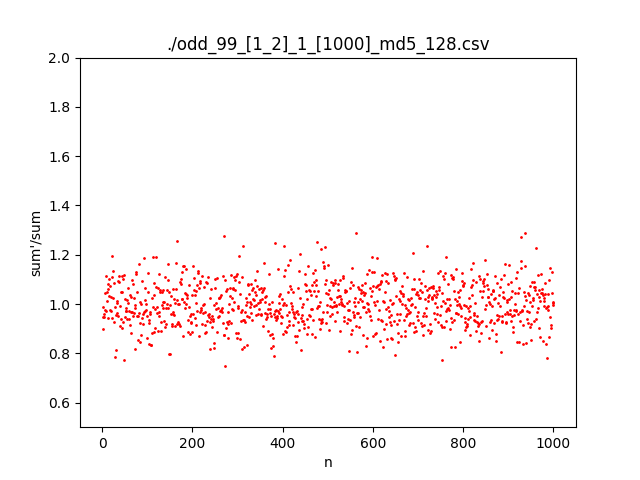
\includegraphics[width=1.0\linewidth, height=5cm]{odd_99_1_2_1_1000/odd_99_1_2_1_1000_md5_128.png}
        \caption{$m = 128$}
        \label{fig:subim2}
    \end{subfigure}
    \begin{subfigure}{0.5\textwidth}
        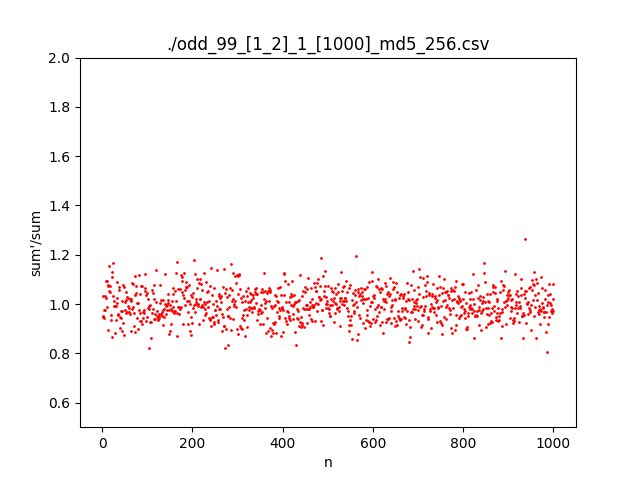
\includegraphics[width=1.0\linewidth, height=5cm]{odd_99_1_2_1_1000/odd_99_1_2_1_1000_md5_256.png}
        \caption{$m = 256$}
        \label{fig:subim2}
    \end{subfigure}

    \caption{Wykresy przedstawiają wyniki algorytmu dla różnej ilości rejestrów gdy wartości cech są w większości podobne, lecz zawierają wartości odstające. Wykorzystano stosunek, $1\%$. Wykorzystany algorytm: \texttt{md5}.}
    \label{fig:uniform_md5}
\end{figure}

\begin{figure}[H]
    \begin{subfigure}{0.5\textwidth}
        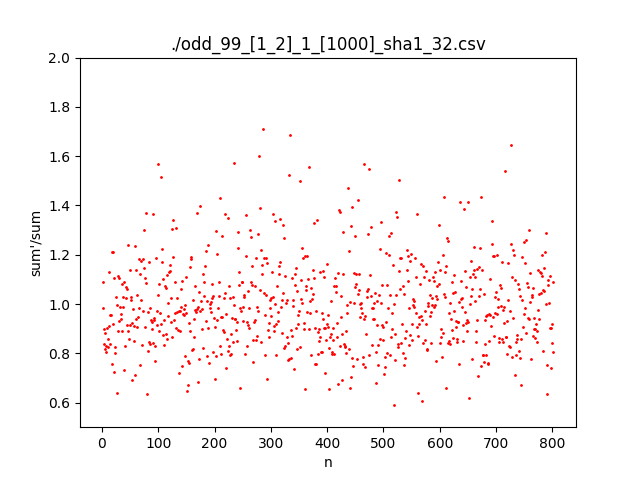
\includegraphics[width=1.0\linewidth, height=5cm]{odd_99_1_2_1_1000/odd_99_1_2_1_1000_sha1_32.png}
        \caption{$m = 32$}
        \label{fig:subim1}
    \end{subfigure}
    \begin{subfigure}{0.5\textwidth}
        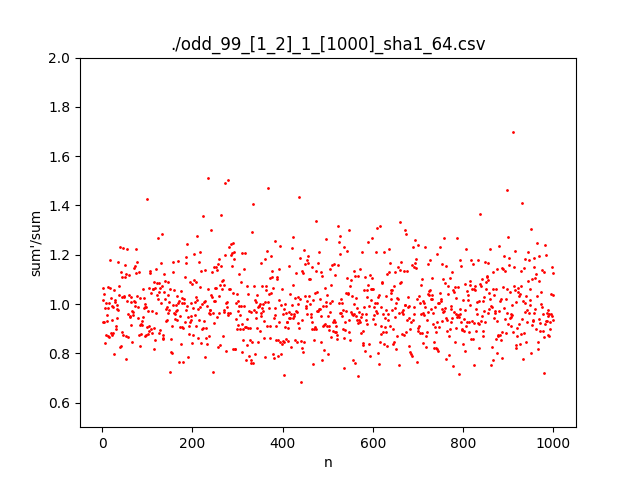
\includegraphics[width=1.0\linewidth, height=5cm]{odd_99_1_2_1_1000/odd_99_1_2_1_1000_sha1_64.png}
        \caption{$m = 64$}
        \label{fig:subim1}
    \end{subfigure}
    \begin{subfigure}{0.5\textwidth}
        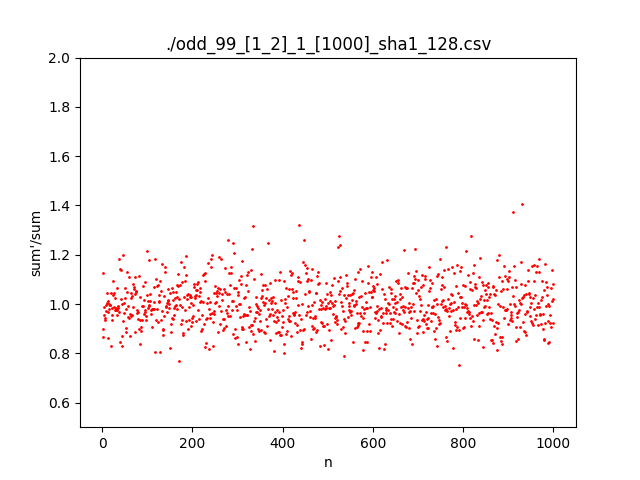
\includegraphics[width=1.0\linewidth, height=5cm]{odd_99_1_2_1_1000/odd_99_1_2_1_1000_sha1_128.png}
        \caption{$m = 128$}
        \label{fig:subim2}
    \end{subfigure}
    \begin{subfigure}{0.5\textwidth}
        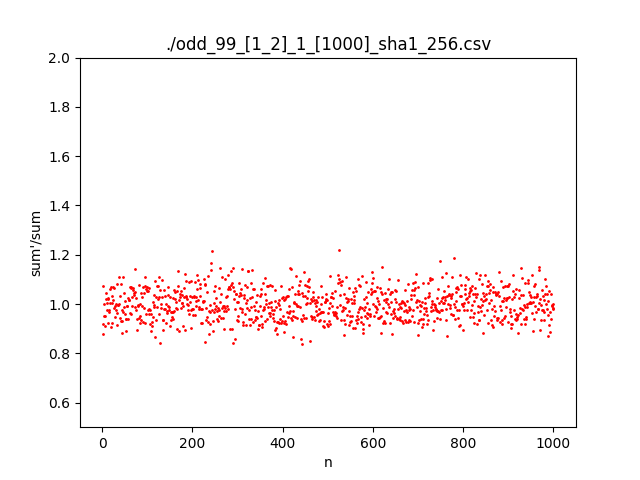
\includegraphics[width=1.0\linewidth, height=5cm]{odd_99_1_2_1_1000/odd_99_1_2_1_1000_sha1_256.png}
        \caption{$m = 256$}
        \label{fig:subim2}
    \end{subfigure}

    \caption{Wykresy przedstawiają wyniki algorytmu dla różnej ilości rejestrów gdy wartości cech są w większości podobne, lecz zawierają wartości odstające. Wykorzystano stosunek, $1\%$. Wykorzystany algorytm: \texttt{sha1}.}
    \label{fig:uniform_sha1}
\end{figure}

\begin{figure}[H]
    \begin{subfigure}{0.5\textwidth}
        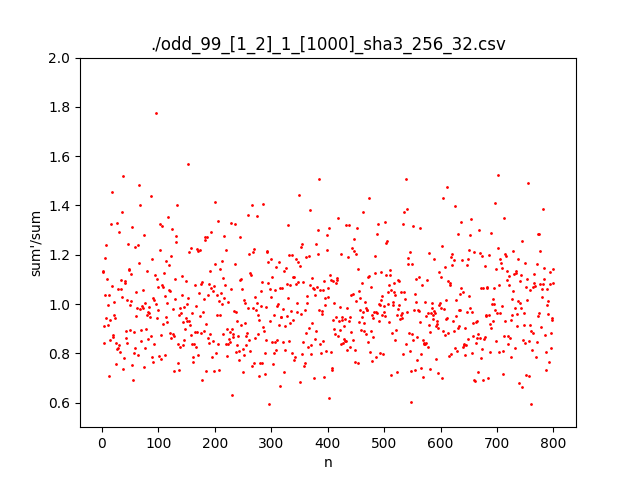
\includegraphics[width=1.0\linewidth, height=5cm]{odd_99_1_2_1_1000/odd_99_1_2_1_1000_sha3_256_32.png}
        \caption{$m = 32$}
        \label{fig:subim1}
    \end{subfigure}
    \begin{subfigure}{0.5\textwidth}
        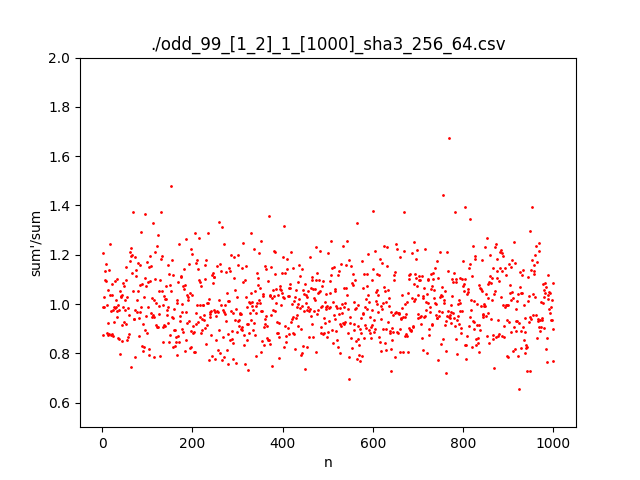
\includegraphics[width=1.0\linewidth, height=5cm]{odd_99_1_2_1_1000/odd_99_1_2_1_1000_sha3_256_64.png}
        \caption{$m = 64$}
        \label{fig:subim1}
    \end{subfigure}
    \begin{subfigure}{0.5\textwidth}
        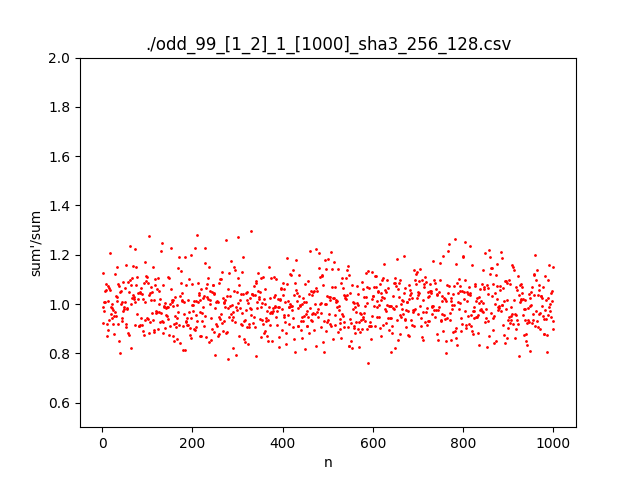
\includegraphics[width=1.0\linewidth, height=5cm]{odd_99_1_2_1_1000/odd_99_1_2_1_1000_sha3_256_128.png}
        \caption{$m = 128$}
        \label{fig:subim2}
    \end{subfigure}
    \begin{subfigure}{0.5\textwidth}
        \includegraphics[width=1.0\linewidth, height=5cm]{odd_99_1_2_1_1000/odd_99_1_2_1_1000_sha3_256_256.png}
        \caption{$m = 256$}
        \label{fig:subim2}
    \end{subfigure}

    \caption{Wykresy przedstawiają wyniki algorytmu dla różnej ilości rejestrów gdy wartości cech są w większości podobne, lecz zawierają wartości odstające. Wykorzystano stosunek, $1\%$. Wykorzystany algorytm: \texttt{sha3}.}
    \label{fig:uniform_sha3_256}
\end{figure}


\end{document}